\section{Preferential attachment: \emph{"The rich get richer"}}
\label{sec:burstiness}

The term \textit{burstiness} describes the fact that some events appear in bursts, \textit{i.e.} once they appear, they are more likely to appear again. The notion of burstiness is similar to the one of aftereffect of future sampling \cite{feller_68}, which describes the fact that the more we observe an event, the higher the expectation to find new occurrences of this event. In (social) network studies, the burstiness effect is alos referred to as \textit{preferential attachment}\footnote{A.L. Barab\'asi, for example, uses the term \textit{preferential attachment} in \cite{barabasi1999emergence}, and \textit{burstiness} in \cite{barabasi_burst}.}: a node with many connections is more likely to have new connections than a node with few connections. To take into account this behavior, in the network generative model  (BA) \cite{albert2002statistical} model, a node is connected to an existing target node with a probability proportional to the number of links of the target node. This leads to scale-free networks that are characterized by a heavy tailed degree distribution, which can be approximated by a power law distribution such that the fraction of nodes $\pr(d)$ having a degree $d$ follows a power law $d^{-\gamma}$, where $\gamma$ typically ranges between 2 and 3~\cite{barabasi1999emergence}. 

Burstiness has been studied in different fields, in particular in computational linguistics and information retrieval to characterize word occurrences \cite{church1995poisson}. In these domains, simple definitions of burstiness, that directly capture the fact that a probability distribution is bursty if the probability of generating a new occurrences of an event increases with the number of occurrences of this event, have been proposed\cite{clinchant2008bnb,clinchant2010information}. We rely here on the discrete version of theses definitions, which takes the following form:
%
\begin{definition}[Burstiness]
	A discrete distribution $\pr$ is bursty if and only if, for all integers $(n, n')$, $n > n'$ :
	\begin{equation}
	\pr(X \geq n+1 \mid X \geq n) > \pr(X \geq n'+1 \mid X \geq n') \nonumber
	\end{equation}
	where $X$ denotes a random variable.
\label{def:burst}
\end{definition}
%
In the context of social networks, the notion of burstiness, or preferential attachment, appears at different levels: (a) a global preferential attachment level that characterizes the degree distribution of nodes in the network, (b) a local preferential attachment level that characterizes the degree distribution of nodes within communities, and (c) a feature burstiness level that characterizes the distributions of nodes among latent features. The feature burstiness characterize the importance of each features depending on how much they are represented within each nodes. We provide below a formal definition of these elements.
%

In the following we will use the notation $\Delta_n\ $ as referring to a discrete differentiation on $n$ such that for any series $b_n$ on has:
\begin{equation*}
    \Delta_n\  b_n = b_{n+1} - b_n
\end{equation*}


\begin{definition}[Burstiness in social networks]
Let $i$ be a node in a social network $G=(V,E)$, and let $d_i$ denote its degree. Furthermore, let $\mathcal{M} \in \{\M_e, \M_g\}$ be a link prediction model as defined in Section~\ref{sec:models}: 
\begin{description}
\item[(i)] \emph{Global Preferential Attachment}: we say that $\mathcal{M}$ satisfies the global preferential attachment iff, for any node $i \in V$, we have:
 \begin{equation}
 \Delta_n\  \pr(d_i \geq n+1 | d_i \geq n,  \M) > 0
 \end{equation}
\item[(ii)] \emph{Local Preferential Attachment}: we say that $\mathcal{M}$ satisfies the local preferential attachment iff, for any node $i \in V$  belonging to a block $c$, we have:
  \begin{equation}
 \Delta_n\  \pr(d_{i,c} \geq n+1 | d_{i,c} \geq n,  \M) > 0
 \end{equation}
  Where $d_{i,c}$ denotes the degree of node $i$ inside the block $c$.
\item[(iii)] \emph{Feature Burstiness}: we say that $\mathcal{M}_e$ satisfies the feature burstiness effect, iff, for any feature $k$ in the network,   
  \begin{equation}
	\Delta_n\  \pr(f_{\bm{.}k} \geq n+1 | f_{\bm{.}k} \geq n,  \M) > 0
  \end{equation}
   Where $f_{\bm{.}k}$ denotes the sum of the k-th features over all network's node such that $f_{\bm{.}k} = \sum_{j=0}^{N-1} f_{jk}$.
\end{description}
\label{def:burst-soc-net}
\end{definition}
%
The definitions of the different properties based on the burstiness involves inequalities over the degree who are not easy to handle in general. Thus, we study in the following a way to formulate it in a more convenient form. Let us first define an appropriate random structure for exchangeable networks.

\begin{definition}
	Let $n$ and $N$ be two natural integer such that $N \geq n$. We define the random structure $x^{N,n}$ as a set of $N$ binary value having $n$ elements active (equal to one) and such that $\sum_{i=0}^N P(x^{N,i}) = 1$.
	\label{def:rd_struct}
\end{definition}

This definition enables the link between the random variable $n$ being a integer (a node degree for example) and the structure that is homogeneous to a row (or a column) in a adjacency matrix that contains in some way this integer.

\begin{theorem}[Burstiness to Global Preferential Attachment] \label{th:burst_exch}
	 A degree distribution $p(d_i=n)$ of any node $i$ in a jointly exchangeable graph $G(V,E)$ is bursty iff :
	\begin{equation}
	 \Delta_n\   p(y_{ij}=1 | d_i^{N,n}) \frac{N-n}{n+1} > 0
	\end{equation}

\end{theorem}

\begin{proof} 	\label{proof:glob}
	First we recall that for a jointly exchangeable graph, we have that:
	\begin{equation*}
	\p(y_{ij}: (i,j) \in V^2) = \p(y_{\pi(i)\pi(j)}: (i,j) \in V^2)
	\end{equation*}
	For any permutation $\pi$ of the integer $\{1,..,n\}$. Furthermore it can be show that $ \pr(d_i \geq n'+1 \mid d_i \geq n')$ and $\frac{\p(d_i=n+1)}{\p(d_i=n)}$ vary in the same direction with $n$ (Clinchant 2006). Under the exchangeability assumptions, one can write that:
	
	\begin{align*}
	 b_n=\frac{\p(d_i=n+1)}{\p(d_i=n)} = \frac{\dbinom{N}{n+1} p(d_i^{N,n+1})}{\dbinom{N}{n} p(d_i^{N,n})}
	\end{align*}
 Applying a product rule, we have that:
	
	\begin{equation*}
	b_n = \frac{N-n}{n+1} \p(y_{ij}=1 | d_i^{N,n})
	\end{equation*}
	
	The differential is then equal to:
	\begin{align*}
	&\Delta_n\  b_n= b_{n+1} - b_n  \\
	&= \frac{N-n-1}{n+2} \p(y_{ij}=1 | d_i^{N,n+1}) - \frac{N-n}{n+1} \p(y_{ij}=1 | d_i^{N,n})
	\end{align*}
	
	The burstiness property is satisfied  $\forall n \in \mathbb{N}$ iff:
	\begin{align} \label{b-theorem}
	&\Delta_n\  b_n > 0 \iff \nonumber \\
	& \frac{(n+1)(N-n-1)}{(n+2)(N-n)}\p(y_{ij}=1 | d_i^{N,n+1})  > \p(y_{ij}=1 | d_i^{N,n})
	\end{align}
	
\end{proof}

In figure \ref{fig:bp} we represent the values of the coefficient of the left part in equation \eqref{b-theorem} in function of $n$ with $N$ equal to 100.
	
The study of this series gives hint about how and when the distribution of the degree would be bursty. We can show that this series is less than 1 with a maxima at $(N-2)/2$ and its symmetric around this extrema for $n \in [0, N-2]$. One can see that the burstiness effect for exchangeable sequence with finite capacity $N$ will collapse for a small number of observation or when the number of observations get closer to the capacity.
	
	\begin{figure}[h]
		\centering
		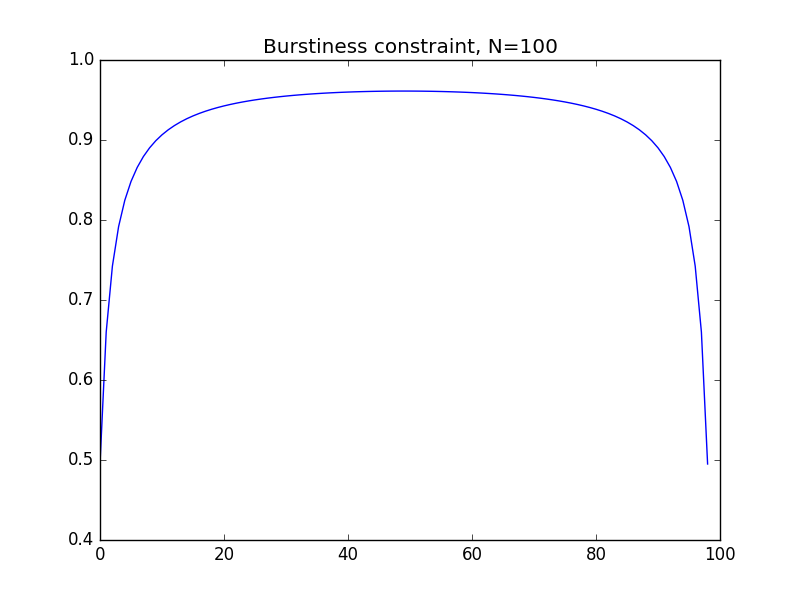
\includegraphics[scale=0.4]{\lpath/img/bp}
		\caption{This plot represent the series that constraints the predictive distribution for the burstiness effect in exchangeable graph for N=100 (100 nodes)}.
		\label{fig:bp}
	\end{figure}



\paragraph{Case of linear predictive distribution}~\\

A typical form of the predictive distribution $\p(y_{ij}=1 | d_i^{N,n})$ is a linear function of the sufficient statistics of the observations (see \ref{prop:diaconis}). We now study the burstiness effect in this case with regards to theorem \ref{th:burst_exch}.

We suppose that the predictive distribution has a linear form such that:

\begin{equation*}
p(y_{ij}=1 | d_i^{N,n}) = an+b
\end{equation*}  
Where $n$ is a positive integer and $a$ and $b$ two positive real numbers. From theorem \ref{th:burst_exch} one has the following condition in order to satisfy the global preferential attachment:

\begin{equation} \label{eq:polynom}
\frac{-an^2 -3an +a(N-1)-b(N+1)}{(n+2)(N-n)} > 0 
\end{equation}
The denominator of this equation strictly positive for $n \in [0, N-1]$. The condition depends then on the sign of the numerator. This polynomial of degree 2 admits 2 roots denoted $n_-$ and $n_+$ given by:
\begin{align*}
n_+ &= \frac{-3a + \sqrt{a(4N(a-b)+5a-4b)}}{2a} \\
n_- &= \frac{-3a - \sqrt{a(4N(a-b)+5a-4b)}}{2a} \\
\end{align*}

If we study the polynomial on the support of the real numbers, we can see that it is negative when $n$ tends to $+\infty$ and $-\infty$. Thus it takes positive values between the roots if they exists. The condition of existence is that the positivity of the roots:
\begin{equation*}
a(4N(a-b)+5a-4b) > 0 \iff b < a \frac{4N+5}{4N+4}
\end{equation*}

Furthermore, only one roots can be positive under the following constraint:
\begin{align*}
\sqrt{a(4N(a-b)+5a-4b)} > 3a \iff a\frac{N-1}{N+1} > b
\end{align*}

If such constraint is satisfied, the polynomial admits positive values for $n \in [0, n_+]$. This development shows that for certain form of the predictive distribution, the burstiness property can not be satisfied for all integers $n$. However a bursty phenomenon can exists on an interval $[0, n_+]$ whose upper bound is determined by the hyperparameters of the model.

We now study the local preferential attachments by formulating a second theorem that enable link from the definition to the predictive distribution. We will show that both theorem are related in a simple and natural way.

\begin{theorem}[Burstiness to Local Preferential Attachment] \label{th:burst_local}
    Let $\M_g$ be a network model of a jointly exchangeable graph $G(V,E)$. Let $N^c$ and $N^r$ be two integers such that the former is the number of nodes in a block $c \in \{0,.., K-1\}$, and the second the number of nodes not being in $c$, such that $N^c+N^r = N$. A local degree distribution $p(d_{i,c}=n)$ for any node $i$ in $c$ is bursty iif:
	
\begin{equation}
\Delta_n\   p(y_{ij}=1 | d_{i,c}^{N^c,n}) \frac{\sum_{r=0}^{N^r}\dbinom{N}{n+1+r} p(d_{ir}^{N^r,r})}{\sum_{r=0}^{N^r} \dbinom{N}{n+r} p(d_{ir}^{N^r,r}) } > 0
\end{equation}
	
\end{theorem}

\begin{proof}
The exchangeable graph $G(V,E)$ contains $|V|=N$ nodes. Thus in the context of the local preferential attachment we consider the degree of a node $i$ belonging to the block $c$ containing $N^c$ nodes. The degree of this node within this block is denoted by $d_{i,c}$ and the  number of node out of the block $c$ is equal to $N^r = N - N_c$. We can write the distribution of the degree inside that block by marginalizing the possible edges between node $i$ and the nodes that are not in $c$. We have:
\begin{equation*}
p(d_{ic}=n) = \sum_{r=0}^{N^r} p(d_{ic}=n,d_{ir}=r)
\end{equation*}
From exchangeable assumptions, it follows:

\begin{equation*}
p(d_{ic}=n) = \sum_{r=0}^{N^r} \dbinom{N}{n+r} p(d_{ic}^{N^c, n},d_{ir}^{N^r, r})
\end{equation*}

Under the assumptions that each local random parameters are i.i.d, we can separate the joint distribution: ( \textcolor{red}{on peut ouvrir la distribution avec les F et les Phi, pour voir que ca marche pour IMMSB EDIT: je pense que c'est en fait vrai pour ILFM aussi, le point clé etant que les poid $\phi_{kk}$ sont indépendement distribue ce qui fait que l'on peut séparer les partie correspondantes a chaque block.)}: 

\begin{align*}
p(d_{ic}=n) &= \sum_{r=0}^{N^r} \dbinom{N}{n+r} p(d_{ic}^{N^c, n}) p(d_{ir}^{N^r, r}) \\
 &=  p(d_{ic}^{N^c, n})\sum_{r=0}^{N^r}   \dbinom{N}{n+r} p(d_{ir}^{N^r, r})
\end{align*}

Finally by applying the burstiness properties as in proof \ref{proof:glob}, and product rule we can formulate the burstiness in function of the predictive distribution:

\begin{equation} \label{eq:29}
b_n =  p(y_{ij}=1 | d_{i,c}^{N^c,n}) \frac{\sum_{r=0}^{N^r}\dbinom{N}{n+1+r} p(d_{ir}^{N^r,r})}{\sum_{r=0}^{N^r} \dbinom{N}{n+r} p(d_{ir}^{N^r,r}) }
\end{equation}

\end{proof}

\textcolor{red}{Open Probem:  Je n'ai pas encore réussi à solver le ratio ci-dessus permettant de conclure sur le local bursty}


We can see that in the case where $N^r=0$ equation \eqref{eq:29} reduce to:
\begin{align*}
b_n &= p(y_{ij}=1 | d_{i,c}^{N^c,n}) \frac{\dbinom{N}{n+1}}{ \dbinom{N}{n} } \\
 &=  p(y_{ij}=1 | d_{i,c}^{N^c,n}) \frac{N-n}{n=1}
\end{align*}

And in this case $N^c=N$. This show that the results of theorem \ref{th:burst_exch} and \ref{th:burst_local} are equivalent in this case which is sounds since $N^r=0$ means that we consider link inside only one block, and so it is like evaluating the global preferential attachment.
%\begin{corollary}
%	A degree distribution  $p(d_i=n)$ of any node $i$ in a jointly exchangeable graph $G(V,E)$ such that it admits a predictive distribution of the form $\p(y_{ij}=1 | d_i^{N,n}) = an+b$, is bursty iff:
%Polynome solution, constraint on the positive roots, a, b > ...
%\end{corollary}

We now apply the previous results to characterize the preferential attachments effect in social networks.


\begin{proposition}
    The IMMSB model satisfies the local preferential attachment property in the generative version $\M_g$. \textcolor{red}{Pour conclure et raffiner la proposition, nous devons nous entendre sur les theorem V.1 et V.2 ( But theorem V.1 doesn't account for simulation that are always bursty with regards to the degree distribution.)}
\end{proposition}

\begin{proof}
In the generative IMMSB model, one can write in the general case the predictive distribution conditioned by $d_i^{N,n}$ has follows:

\begin{equation} 
p(y_{ij} = 1 | d_i^{N,n}, \mathcal{M}_g) = \int_{\Theta} p(y_{ij}=1|\Theta) \frac{p(d_i^{N,n} | \Theta)}{p(d_i^{N,n})} p(\Theta) d\Theta \nonumber
\end{equation}

Recall that in IMMSB the interaction $y_{ij}$ between two nodes $i$ and $j$ depends on their respective block assignments, and consequently, two nodes belongs to the same block $c$ if they took the same assignments (assignments are indicated in the variable $z$ drawing from the latent features in the generative process.).

In the context of the local preferential attachment property we consider only the relation inside this block $c$ and the predictive distribution is given by:

\begin{align*} \label{eq:sum}
&p(y_{ij} = 1 | d_{ic}^{N^c,n}, \mathcal{M}_g)  \\
&=  \frac{ \int_{\phi_{c}} p(y_{ij}=1|\phi_{c}) p(d_{ic}^{N,n} | \phi_{c}) p(\phi_{c}) d\phi_{c}}{\int_{\phi_{c}} \p(d_{ic}^{N^c,n} | \phi_{c}))       p(\phi_{c}) d\phi_{c}}   \\
&= \frac{\int_{\phi_c} \phi_c^{n+1}(1-\phi_c)^{N^c-n} \phi_c^{\lambda_1-1} (1-\phi_c)^{\lambda_0-1} d\phi_{c}}{\int_{\phi_c} \phi_c^{n}(1-\phi_c)^{N^c-n} \phi_c^{\lambda_1-1} (1-\phi_c)^{\lambda_0-1} d\phi_{c}} \\
&= \frac{ \text{B}(n+1+\lambda_1, N^c-n+\lambda_0) }{\text{B}(n+\lambda_1, N^c-n+\lambda_0)} \\
&= \frac{n+\lambda_1}{N^c + \lambda_1 +\lambda_0}
\end{align*}

where $\text{B}()$ is the beta function. Given the last equation it's obvious that the  predictive likelihood is linear with $n$.

    \paragraph{\textcolor{red}{Theorem \ref{th:burst_exch} Framework }}~\\

In particular,  let's now suppose that the predictive distribution takes this specific linear according to parameters :
\begin{equation*}
p(y_{ij}=1 | d_i^{N,n}) = \frac{n+\lambda_1}{N+\lambda_1+\lambda_0}
\end{equation*}
    This is equivalent to solving the polynomial \eqref{eq:polynom} for $a=1$ and $b=\lambda_1$. In such a case, the burstiness effect will be present in the subset $n \in \{0, n_+\}$ iff the following holds:
\begin{equation*}
\lambda_1 < \frac{N-1}{N+1}
\end{equation*}

    \paragraph{\textcolor{red}{Theorem \ref{th:burst_local} Framework }}~\\

    $\frac{\sum_{r=0}^{N^r}\dbinom{N}{n+1+r} p(d_{ir}^{N^r,r})}{\sum_{r=0}^{N^r} \dbinom{N}{n+r} p(d_{ir}^{N^r,r})}$  \textcolor{red}{ ? }

\end{proof}

\begin{proposition}
    The ILFM model does not satisfy the local preferential attachments in the generative model $\M_g$. \textcolor{red}{ meme question qu'audessus pour conclure cette proposition}
\end{proposition}

\begin{proof}
As for IMMSB proof, we only consider the relations  that occur inside block $c=\{k,k\}$, thus we note $N^c$ the total number of nodes being in the block $c$. In ILFM being in the block $c$ means that we evaluate the predictive distribution by only considering the column $c$ of the feature matrix. We can interpret this operation as looking the connections pattern when only the contribution of the feature $c$ is at work. One can write the predictive distribution inside this block as follows:

\begin{align*}
&\p(y_{ij}=1 | d_{ic}^{N^c,n}, \M_g)  \\
&=  \frac{ \int_{\phi_{c}} p(y_{ij}=1|\phi_{c}) p(d_{ic}^{N,n} | \phi_{c}) p(\phi_{c}) d\phi_{c}}{\int_{\phi_{c}} \p(d_{ic}^{N^c,n} | \phi_{c}))       p(\phi_{c}) d\phi_{c}} \\
&= \frac{ \int_{\phi_{c}} \sigma(\phi_c) \sigma(\phi_c)^n (1-\sigma(\phi_c))^{N^c-n}     p(\phi_{c}) d\phi_{c}}{\int_{\phi_{c}}  \sigma(\phi_c)^n (1-\sigma(\phi_c))^{N^c-n}      p(\phi_{c}) d\phi_{c}} \\
&= \frac{ \int_{\phi_{c}} \sigma(\phi_c) \sigma(\phi_c)^n \sigma(-\phi_c)^{N^c-n}     p(\phi_{c}) d\phi_{c}}{\int_{\phi_{c}}  \sigma(\phi_c)^n \sigma(-\phi_c)^{N^c-n}      p(\phi_{c}) d\phi_{c}} \\
&= \frac{ \int_{\phi_{c}} \sigma(\phi_c) (\frac{\sigma(\phi_c)}{\sigma(-\phi_c)})^n \sigma(-\phi_c)^{N^c}     p(\phi_{c}) d\phi_{c}}{\int_{\phi_{c}}  (\frac{\sigma(\phi_c)}{\sigma(-\phi_c)})^n \sigma(-\phi_c)^{N^c}     p(\phi_{c}) d\phi_{c}} \\
&= \frac{ \int_{\phi_{c}} \frac{\exp(n\phi)}{1+\exp(-\phi)} \frac{\exp(-N\phi)}{(1+\exp(-\phi))^{N^c}}  p(\phi_{c}) d\phi_{c}}{\int_{\phi_{c}}  \exp(n\phi) \frac{\exp(-N\phi)}{(1+\exp(-\phi))^{N^c}}   p(\phi_{c}) d\phi_{c}} \\
&= \frac{ \int_{\phi_{c}} \exp(\phi(n-N)) \sigma(\phi)^{N+1} p(\phi_{c}) d\phi_{c}}{\int_{\phi_{c}} \exp(\phi(n-N)) \sigma(\phi)^{N} p(\phi_{c}) d\phi_{c}} \\
\end{align*}

\begin{equation}
\int_{\phi_{c}} \exp(\phi(n-N)) \sigma(\phi)^{N+1} p(\phi_{c}) d\phi_{c} \ ?
\end{equation}


With $\sigma(\phi) = \frac{1}{1+\exp(-\phi)}$ and $\p(\phi) = \mathcal{N}(0, \sigma_w)$.



\textcolor{red}{not ended yet...same issue than the local case for IMMSB for the choice of the theorem.}
\end{proof}

We now turn to the mode $\M_e$. It is important to note here the fact that the probability $\pr(y_{ij}=1 \mid d_i \ge n, \M_e)$ increases with $n$ is equivalent to the fact that the probability $\pr(d_{i} \ge n+1 \mid d_i \ge n, \M_e)$ increases with $n$. Indeed:


\begin{align}
&\pr(d_{i} \ge n+1 \mid d_i \ge n, \M_e) \nonumber \\
&= 1 - \prod_{j \notin \mathcal{V}(i)} P(y_{ij} = 0 \mid d_i \ge n, \M_e) \nonumber \\
&= 1 - \prod_{j \notin \mathcal{V}(i)} (1 - P(y_{ij} = 1 \mid d_i \ge n, \M_e)) \nonumber
\end{align}


Hence $\pr(d_{i} \ge n+1 \mid d_i \ge n, \M_e)$ and $P(y_{ij} = 1 \mid d_i \ge n, \M_e)$ vary in the same direction. The same development holds for $\pr(y_{ij}=1 \mid d_{i,c} \ge n, \M_e)$. The above definitions, characterizing probabilistic link models in the mode $\M_e$ according to burstiness in social networks, are thus directly related to the general definition of burstiness given in Definition~\ref{def:burst}.


\begin{proposition}
	The ILFM and IMMSB models do not satisfy the global and local preferential attachments in the mode $\M_e$.
\end{proposition}

The proof of this statement is trivially true in the sens that given $\mat{F}$ and $\mat{\Theta}$, the likelihood is fully determined and hence do not depend on new links being generated. More precisely one has:
\begin{align*}
\p(y_{ij}=1| d_i \ge n, \M_e) &= \p(y_{ij}=1| \M_e)\\
&= \mat{\hat{f}}_{i} \mat{\hat{\Phi}} \mat{\hat{f}}_j^\top
\end{align*}
The predictive likelihood does not depend on $n$ and hence the burstiness is not satisfied. The same development holds for the local preferential attachment by indexing variables by the related block $c$.

One can note that, despite this result, the inference procedure of the posterior distribution will be likely to produce latent features that fit  the burstiness present in the data (if present) as reported in section \ref{sec:experiments}. This is particularly visible on the predictive likelihood for IMMSB which take the following form (see details in appendix \ref{sec:append}):
\begin{equation*} \label{eq:ppp}
p(y_{ij}=1 | \M_e)\propto \sum_{kk'} \frac{M_{(kk')1} + \lambda_1}{M_{(kk')\bm{.}} + \lambda_0 + \lambda_1}  (N_{ik} + \alpha\beta_k ) (N_{jk} + \alpha\beta_k)
\end{equation*}   
One can see that the features that are associated with the weights that cumulate number of observed links will be more likely to generate new links. In the case of ILFM the mixing between feature and weight is less clear since the non-conjugacy produce no close relation between the posterior and the sufficient statistics of the data (ie the degrees count). Nevertheless, the predictive analysis in section \ref{sec:experiments} shows that IMMSB outperform ILFM on bursty networks.

\begin{proposition} \label{prop:diaconis}
    ILFM model satisfy the burstiness effect for $n<n_+$ such that $n_+ \sim \sqrt{N}$  if $N>>0$ \\
    IMMSB model satisfy the burstiness effect for feature $k$, iif $n<n_+$ and $\alpha_k<\frac{N-1}{N+1}$ such that $n_+ \sim \sqrt{N(1-\lambda_1)}$ if $N(1-\lambda_1)>>0$ 
\end{proposition}

\begin{proof}
The Diaconis-Ilvisaker theorem \cite{diaconis1979conjugate} state \emph{'subject to regularity conditions, the conjugate priors typically used satisfy, and are characterized by, a  similar relation of posterior linearity'}:
\begin{equation}
\E_\Theta[\E_{X|\Theta}[X\mid \Theta] \mid X=x] = ax+b \quad \text{for} \quad x=0,1,2,... \nonumber
\end{equation}

Especially, the Dirichlet Process and the Indian Buffet Process, as prior for the latent features, are typically build on the suitable conjugate distribution, respectively a Dirichlet-Multinomial and a Beta-Bernoulli. Furthermore, this claim is highlighted by the Gibbs update the characterize their predictive distribution of feature and corroborate the feature burstiness effect:
\begin{align*} 
&\p(f_{ik} = 1 | F^{-ik}) = \frac{m_k^{-ik}}{N} \qquad \hspace{20pt} \text{ILFM feature update} \nonumber \\
&\p(f_{ik} = 1 | F^{-ik}) = \frac{n_{ik}^{-z_{ij}}+\alpha_k}{N+\alpha_.} \qquad \text{IMMSB feature update} \nonumber \\
\end{align*}

Where the $m_k^{-ik}$ described the number of elements that have the $k$-iem feature active except for element $i$, similarly $n_{ik}^{-z_{ij}}$ represents the number of times that $i$ was assigned to $k$ except for relation $(ij)$ (block membership are jointly sampled in MMSB).

By applying theorem \ref{th:burst_exch} for linear predictive distribution, we showed show that the burstiness is true until $n_+$ if the following polynomial admit a positive root:
\begin{equation*}
	 an^2 + 3an - a(N-1) + b(N+1) = 0
\end{equation*}

    In the case of ILFM and IMMSB, it is equivalent to solve the polynomial with $a=1$, $b=0$ for ILFM and $a=1$, $b=\alpha_k$ for IMMSB. The positive root arise in this case if $b < \frac{N-1}{N+1}$, which determines $n_+$. Thus for the ILFM, the root is only positive while for IMMSB, the positive root arise if $\alpha_k < \frac{N-1}{N+1}$. Moreover, when the number of nodes increase such that $N >> 0$, the born become $n_+ \sim \sqrt{N}$. The asymptotic born is the same for IMMSB if $\alpha_k << 1$.
\end{proof}

This proposition suggest that HDP and IBP are admissible priors in order to satisfy a burstiness effect on the latent features until a reasonable born. This born is asymptotically  (with a mild condition on IMMSB), the square root of the number of nodes. Note that the constraint that we find for the condition over the hyperparameters of the truncated Dirichlet (for IMMSB), directly traduce the well know fact that the more the parameters of a Dirichlet distribution are small the more the sample will be sparse. Or equivalently, the distribution will be concentrated on the corners of its simplex.

\subsection{Empirical Illustration}

We illustrate the burstiness results by generating 3 random networks for each of both models. We report it in figure \ref{fig:gen_burst}. We use the 3 same settings for IMMSB  than those in the previous section. For ILFM  we use the following 3 settings: (column 1:$\alpha=1,  \lambda_1=\lambda_2=1$ , column 2:$\alpha=0.1, \lambda_1=\lambda_2=1$, column 3: $\alpha=1, \lambda_1=\lambda_2=10$) and we fix $\sigma_w=1$ and again $N=1000$.

Each row of the two sets of figures represents the three following measures who corresponds respectively to the global preferential attachment, the local preferential attachment and the feature burstiness:
\begin{itemize}
    \item First row: we measure the overall degree distributions; We report the average and standard deviation of the degree distribution in a linear scale for each generated network.
    \item Second row: we measure the local degree distribution on a log-log scale:
        \begin{itemize}
            \item for IMMSB, each network has an associated membership tensor $Z$, that indicates the membership of nodes for each  interactions. In order to draw the local degree distribution for a block $c$, we reduce the adjacency matrix in order to retain only the links that occurs inside a block $c$. The local degree distribution is thus computed on the reduce adjacency matrix $Y_c = Y \otimes (Z_i^c \times Z_j^c)$ where $\otimes$ is the hadamard product and $\times$ the outer product. $Z_i^c$ is the membership matrix of a nodes $i$ such that $Z_{ik}^c=0$ if $k\neq c$ (links that occurs outside $c$ will be ignored).
            \item for ILFM, each node is associated with a fix feature vector; the local degree distribution for the block $c$ is obtain by taking only the contribution of the features $c$ on the adjacency matrix. Thus, the local degree degree distribution is computed on the reduce adjacency matrix $Y_c = Y \otimes (F_{.c}\times F_{.c})$. 
        \end{itemize}
    \item Third row measure the distribution of the block membership, which directly reflect the feature burstiness. Hence for IMMSB, for a feature $k$, we measure $\sum_{ij} \mathds{1}(Z_{i\rightarrow j} = k, Z_{i\leftarrow j} = k)$ which indicates the number of nodes who were associated to the block $k$. For ILFM the number of nodes associated to a block $k$ is simply $\sum_n F_{nk}$.
\end{itemize}


% not sure it use significantly usefull, because p-value are either 0 or 1 ...
%We provide in annexe (\textcolor{red}{not yet included}),  an goodness of fit for all local degrees distribution that we plotted, in order to quantify the power law hypothesis on the empirical degree distributions. The number of feature is typically too small to evaluate an significant goodness of fit. The protocol is described in section \ref{sec:experiments-busrt}. 

The simulation shows us the following facts about the properties of the models:
\begin{itemize}
	\item For both model the global degree distribution don't exhibit a bursty phenomenon,
	\item The local degree distribution show that IMMSB exhibit a bursty phenomenon which is not the case for ILFM,
	\item Both models exhibits a bursty phenomenon on the feature distribution. This distributions for ILFM has a long tail for all of the 3 settings while for IMMSB, the tail shape is more or less long depending of the $\alpha$ and $\gamma$ parameters.
\end{itemize}

For the case of the global preferential attachment we have no formal proof for the non-compliance of the models, due the non closed form of the evidence in both models, due to the admixture design \textcolor{red}{ref ((Multiple Hypergeometric Functions: Probabilistic Interpretations and Statistical Uses
James M. Dickey )) ce papier est cite dans LDA pour justifier l'inference approxime, mais je n'arrive pas a trouver ca papier !!!}. However, as reported simulations (figure \ref{fig:gen_burst}), we see that the empirical distributions of the overall degrees are clearly non bursty.


\begin{figure*}[ht]
	\centering IMMSB\\
	\minipage{0.27\textwidth}
	\includegraphics[scale=0.27]{\lpath/img/M_g_peaks/figure_1}
	\endminipage
		\minipage{0.27\textwidth}
	\includegraphics[scale=0.27]{\lpath/img/M_g_power_law/figure_1}
	\endminipage
	\minipage{0.27\textwidth}
	\includegraphics[scale=0.27]{\lpath/img/M_g_regular/figure_1}
	\endminipage
		\vspace{-0.29cm}
	\minipage{0.27\textwidth}
	\includegraphics[scale=0.27]{\lpath/img/M_g_peaks/figure_3}
	\endminipage
		\minipage{0.27\textwidth}
	\includegraphics[scale=0.27]{\lpath/img/M_g_power_law/figure_3} 
	\endminipage
	\minipage{0.27\textwidth}
	\includegraphics[scale=0.27]{\lpath/img/M_g_regular/figure_3}
	\endminipage
		\vspace{-0.28cm}
	\minipage{0.27\textwidth}
	\includegraphics[scale=0.27]{\lpath/img/M_g_peaks/figure_5}
	\endminipage
	\minipage{0.27\textwidth}
	\includegraphics[scale=0.27]{\lpath/img/M_g_power_law/figure_5} 
	\endminipage
	\minipage{0.27\textwidth}
	\includegraphics[scale=0.27]{\lpath/img/M_g_regular/figure_5}
	\endminipage

    \vspace{0.2cm}
	 ILFM

	\minipage{0.27\textwidth}
	\includegraphics[scale=0.27]{\lpath/img/ilfm/1/figure_1}
	\endminipage
		\minipage{0.27\textwidth}
	\includegraphics[scale=0.27]{\lpath/img/ilfm/2/figure_1}
	\endminipage
	\minipage{0.27\textwidth}
	\includegraphics[scale=0.27]{\lpath/img/ilfm/3/figure_1}
	\endminipage
		\vspace{-0.29cm}
	\minipage{0.27\textwidth}
	\includegraphics[scale=0.27]{\lpath/img/ilfm/1/figure_3}
	\endminipage
		\minipage{0.27\textwidth}
	\includegraphics[scale=0.27]{\lpath/img/ilfm/2/figure_3} 
	\endminipage
	\minipage{0.27\textwidth}
	\includegraphics[scale=0.27]{\lpath/img/ilfm/3/figure_3}
	\endminipage
		\vspace{-0.28cm}
	\minipage{0.27\textwidth}
	\includegraphics[scale=0.27]{\lpath/img/ilfm/1/figure_5}
	\endminipage
	\minipage{0.27\textwidth}
	\includegraphics[scale=0.27]{\lpath/img/ilfm/2/figure_5} 
	\endminipage
	\minipage{0.27\textwidth}
	\includegraphics[scale=0.27]{\lpath/img/ilfm/3/figure_5}
	\endminipage
    \caption{Generated Networks with IMMSB (top) and ILFM (bottom) for three different settings (same set than for figure \ref{fig:gen_blocks_mmsb}). The top rows measure the global preferential attachment through the overall degree distribution. The middle row measure the local preferential attachment through the local degree distribution. The last row measure the feature burstiness through the block membership distribution.}
	\label{fig:gen_burst}
\end{figure*}

